\documentclass[pageno]{jpaper}

%replace XXX with the submission number you are given from the ISCA submission site.
\newcommand{\IWreport}{2012}

\usepackage[normalem]{ulem}

\begin{document}

\title{
Making Inferences from Individual Behaviour Using Mobile Data}

\author{Tiantian Zha}

\date{}
\maketitle

\thispagestyle{empty}

\begin{abstract}
Patterns within data that results from individual behavior can reveal a great deal of information about the individual's identity and behavior patterns. Merchants with access to consumer data are able to infer highly personal information that was not explicitly disclosed, and that the consumer may not have wanted disclosed. Merely anonymizing is often insufficient; in this paper we explore ways in which we can reconcile anonymized data with known users, and we use similarities between anonymous users and known users to make further inferences about their identity. We also explore ways to connect location, proximity, and relationships between our users. These findings have implications for developing ways to better protect users' privacy. 

\end{abstract}

\section{Introduction}

As data has become increasingly ubiquitous and tools for analyzing them more powerful, companies have been able to gain an edge by learning about their customers' personal information. In this past year, Charlie Duhigg from The New York Times's story on Target's strategy for discovering patterns that signal upcoming childbirth (Duhigg, 2012), as well as Professor Ed Felten's opening speech on this same topic addressed to incoming freshmen, vaulted privacy concerns to the forefront of Princeton campus' collective consciousness. 

\subsection{MIT Reality Mining}
With the growing prevalence of smartphones functioning essentially as an on-the-go computer comes yet another dimension of data that we can mine for information on individual behavior. The MIT Reality Mining project has built a database by tracking the mobile usage of 97 subjects for 9 months. This project was carried out in 2004-2005 using Nokia smartphones, and represents over 500,000 hours of tracking. In addition to gathering phone-usage related information such as phone calls, text messages and location-tracking, researchers also recorded survey information about the individuals' habits, courses of study, and relationships with one another.

\subsection{Existing Research}

Existing research on this data set primarily focuses on mobility profiling and on social networks. 

\subsubsection{Profiling}

Bayir et al. focus on individual paths and created profiles of individual users to understand users' movement patterns. Their models aggregately show that some of the most common paths taken are from home to the Media Lab and from the Media Lab back home. They also tallied the most frequently accessed locations, and found that 15\% of a user's time was spent in a number of places that each account for less than 1\% of the user's time. These spatio-temporal distributions are relevant for making predictions, studying issues related to exposure to the environment, and network planning. 

A number of strategies have been employed to make sense of and give structure to people's daily routines. Eagle and Pentland (2009) describe the approach of decomposing behavior into a set of eigenbehaviors that together can accurately predict future behavior. Given data about the morning, these researchers were able to predict with 79\% accuracy the individual's behaviour for the remainder of the day.

\subsubsection{Social networks}

The database is also a rich source of proximity information that helps us analyze the link between relationshiops and physical proximity. Eagle and Pentland (2004) study the temporal distribution of proximity data, and note the difference in the distribution between friends and acquaintances. Whereas time with friends is distributed over a wide range of hours, proximity with acquaintances is limited to the work day. 

Eagle and Pentland (2009) also investigate the differences in the recall of proximity. They discovered systematic biases in reporting the amount of time spent together, depending on whether the subjects were friends or merely acquaintances. 

\subsection{Privacy Implications}
We hope to similarly identify patterns in the data that allow us to make inferences about individuals based on their behaviour. The degree to which our predictions are accurate has implications for privacy, because it allows a potential attacker to discover more information than was explicitly revealed by the user. We will use different metrics to make predictions, and verify them against the ground truth provided in the Reality Mining data set. 

\subsection{Questions}

The three questions we hope to answer are: 
\begin{itemize}
\item If given existing data on a population of users, and further anonymized data that belongs to one of the users, can we connect this additional data with one of the known identities? This question has implications for the effectiveness of anonymization. 
\item To what extent are users similar to each other? The users in the study come from several different academic programs: can we, using similarity between groups of users, identify who belongs to which program? 
\item What are the different ways in which location can reveal friendships? Can merely the amount of time spent together be an effective tool? 
\end{itemize}

\section{The MIT Reality Mining Database}

Here I will describe how the database is actually organized. There are 2 versions: one in a SQL format, and another one in MATLAB format. For this paper, I mostly used cell phone related data from the SQL file. Ground truth data (user surveys and background information) was more plentiful and clearly organized in the MATLAB file.

\subsection{SQL Database}

This database contains 97 subjects, each uniquely identified by a person\_oid. The data is organized across 10 tables. 
\begin{itemize}
\item \textbf{Cellspan:} Contains a log pertaining to user location. Each entry specifies a starttime, an endtime, a person\_oid, and a celltower\_oid uniquely identifying the cell tower that the user is connected to.
\item \textbf{Cellname:} Contains names that convey the semantic meaning of cell towers, for each individual user. Each entry is uniquely identified by a person\_oid and a celltower\_oid: users are prompted to enter a name for each cell tower the first time that they encounter it. Therefore, many towers have names such as "Media Lab" or "Harvard Square," while some towers have more personal names such as "Veronica's."
\item \textbf{Celltower:} Matches each celltower\_oid to an actual cell tower ID belonging to a telecom company. 
\item \textbf{Callspan:} Records Voice Calls, Short Messages, and Packet Data sent between users. Each communication is between a person\_oid who is part of this experiment, and a phonenumber\_oid which may represent a user in the experiment, or may represent an outside number. No information in this database is provided on reconciling phonenumber\_oids with person\_oids.
\item \textbf{Person:} Contains survey information about the users, such as what program they belong to, which neighborhood they live in, etc.
\item \textbf{Coverspan:} Records when data-logging is occurring. In theory logging should continuously be enabled, but often users switch off their phones or run out of batteries, leading to gaps that are exposed by this data table.
\item \textbf{Devicespan:} Contains information as to when another device is nearby. The person is referred to by their person\_oid. The other device is referred to by a device\_oid.
\item \textbf{Device:} Contains lists of MAC addresses corresponding with a person\_oid and a name. It is unclear how to connect these MAC addresses with device\_oids, or how to connect device\_oids with a person\_oid.
\item \textbf{Activityspan:} Contains a list of starttimes, endtimes, and person\_oids. 
\item \textbf{Phonenumber:} Empty table.
\end{itemize}

\subsection{MATLAB User Information}

This database contains 107 subjects' cell phone usage data and survey data. The same information as above is replicated and is organized by user. Sometimes entries slightly differ (e.g. a given user's Cell\_name names might contain a few extra entries, though the list as a whole unmistakably belongs to the same person).

Additionally, there are 2D matrices indicating relationships between users. Subjects in the experiment are asked to answer which of the other participants they would consider their friends. If users i reports that user j is a friend, then entry[i][j] = 1. Otherwise, the entry is NaN. The matrix is not symmetrical, as there are asymmetric friendships reported. Noteworthy is the fact that here, users are identified by yet a different set of IDs; producers of this data provide an explicit way of translating between the two, but some information is clearly lost as we are translating 107 IDs into 94.

\subsection{Combining the two datasets}

We therefore have 3 sets of IDs to work with: person\_oids used by the SQL database, the 107 IDs used by the MATLAB to organize its users, and the 94 IDs used to describe relationships between users. 

We sync between SQL IDs and MATLAB's 107 user IDs by comparing them across different information fields. Especially relevant are the cellnames that each user gives, and their responses to survey questions. These are highly personalized, and therefore by performing a manual comparison, we can reconcile the two data sets with high confidence. Due to users dropping in / out of the experiment, data is incomplete in some places, fragmented in others. Some information is also slightly inconsistent between the SQL database and the MATLAB database; for example a handful of survey fields may be missing in one version and present in the other, or one list of cellnames might have a couple of additional entries. 

The MATLAB data set provides an explicit conversion array to obtain the relationships ID from the 107 user IDs.

\subsection{Data selection and usage}

Since many of our questions involve comparing the similarity between users, we select portions of data that are readily comparable. Given that we are studying college students, we chose to only use data representing the dates when school is in session: during the summer students return home to DC, New York, and others, which introduces significant irregularities in the data. 

Using web.archive.org's historical copy of MIT's registrar's page, we are able to unearth the duration of the 2004-2005 academic year. We then separate the available data into first semester and second semester; this facilitates experiments using anonymization. 

\section{Anonymization: Finding a needle in a haystack?}

The first question we pose is whether, given existing information about a set of users (e.g. Fall semester cell phone usage patterns) as well as anonymous data for one user from a different time period (e.g. usage patterns from the following Spring semester), can we connect this anonymous user to one of the existing users? In other words, can we identify this user despite the attempt to anonymize? To answer this question, we will measure the degree of similarity between this anonymous user and every known user, and choose the most similar candidate. Specifically, from our data set, we can examine the similarity in location patterns and in call patterns. 

\subsection{Location data}

We compute a user's distribution of locations over time, i.e. what percentage of his or her time each person spends at each location. We then compute the hamming distance between the anonymous user's distribution and each of the known user's distribution. The distance, represented by a floating point number between 0 and 2, is the degree of dissimilarity between 2 users. 

In order to select the most similar user, we sort all users by hamming distance and choose the lowest one. For this analysis, our pool of "known" users had 88 candidates. These are the users who have location data during the 1st semester. We also had 33 distinct valid anonymous users; these are the users who have location data for both semesters so that it is possible to find a correct matching. 

\subsubsection{What constitutes a "location"?}

Crucial to determining how much time each user spends at a location is defining what constitutes a location. We take two approaches. 

The first is to consider each cell tower as a distinct location. The Cellspan table conveniently lists the start time and the end time of a user's stay at this tower. 

However,  in high-density areas, there may be a large number of towers available. Bayir et al. observed that users tend to oscillate between nearby celltowers, and therefore it is possible to consider several towers to be in the same location: users need not move significantly to jump from one tower to another and back (Bayir et al., 2009). 

\subsection{Clustering cell towers}

We borrow Bayir's technique for clustering cell towers into locations.

\subsubsection{Finding oscillating pairs}
These pairs are defined as nodes that occur repeatedly and in alternating order in a path. To locate them, we first find all the paths where a user does not stop at any given location for more than 10 minutes (empirically found to be an accurate value to use to represent a true path). Any location where the user stays for more than 10 minutes consists of an endpoint. Within each path, we find any pairs of 2 towers that alternate 3 times between them (again 3 is an empirically derived number). For example, a path consisting of [a, b, a, b] would yield the oscillating pair (a, b) since we go from a to b, back to a, and back to b for a total of 3 transitions. Similarly, the path [a, b, c, a, b] would also give us (a, b) as an oscillating pair. Transitions do not need to be contiguous, since we assume that the above towers must be close to each other for this alternating to occur. 

Most paths are less than a dozen nodes long, but there are nevertheless many paths that exceed a few dozen nodes. We implemented a brute-force pair-finding algorithm with just one modification. We examine every pair of nodes in a path and check if there are at least three transitions from one to the other. However, we first prune out any node that occurs only once. This drastically reduces the number of pairs that need to be examined.  

\subsubsection{Clustering}
By analyzing each user in this way, we obtain a graph where edges are described by oscillating pairs, and where the weight of each edge is the number of times this oscillating pair occurs within all the data. Bayir does not specify a specific algorithm to use; we used the Markov Clustering algorithm (MCL), which is suitable for this purpose because it requires an undirected graph where the edges represent similarity between nodes. The graph must not be too dense (a lattice), and must not be too sparse (a tree). Our graph, with a small number of cycles among nearby towers, fits these criteria. 

We ran several iterations of this algorithm by varying the inflation number. The inflation number determines how granular the clustering is: a higher inflation number leads to more clusters. We used 1.4, 2.0 (default) and 6.0, a range recommended by the author, yielding us 24526, 25043,  and 25676 clusters respectively. The original number of cell towers is 32656.

\subsubsection{Results}

Two factors primarily affected our accuracy. The higher number of distinct locations improved our guessing rate, as did a larger quantity of data. 


\begin{table}[h!]
  \centering
  \begin{tabular}{|l|l|l|}
    \hline
    \textbf{Clusters} & \textbf{No. of locations} & \textbf{Success rate}\\
    \hline
    \hline
    No clustering & 32656 & 29/33\\
    \hline
    Inflation: 6.0 & 25676 & 19/33\\
    \hline
    Inflation: 2.0 &  25043 & 16/33\\
    \hline
    Inflation: 1.4 & 24526 & 10/33\\ 
    \hline
  \end{tabular}
  \caption{Clustering (number of towers) vs. Accuracy}
  \label{table:formatting}
\end{table}

In the no clustering scenario, we achieved an accuracy rate of 29/33, shown next to the highest number of towers. In subsequent trials with clustering, we see rates of 10/33, 16/33, and 19/33 for inflation numbers of 1.4, 2.0, and 1.6 respectively. All results are a significant improvement over random guessing (which has a 1/88 chance of being correct). 

Another important factor driving the accuracy of our predictions is the amount of data availble. The incorrect answers tended to have been informed by much smaller quantities of data. On average, correctly identified anonymous users had 50\% to 100\% more entries that the incorrectly identified ones. This pattern holds true regardless of whether we clustered.

\begin{table}[h!]
  \centering
  \begin{tabular}{|l|l|l|}
    \hline
    \textbf{Clusters} & \textbf{Correct: no. entries} & \textbf{Incorrect: no. entries}\\
    \hline
    \hline
    No clustering & 12440 & 5403\\
    \hline
    Inflation: 1.4 & 15214 & 10010\\
    \hline
    Inflation: 2.0 &  15572 & 7836\\
    \hline
    Inflation: 6.0 & 14681 & 7388\\
    \hline
  \end{tabular}
  \caption{Quantities of data available for correct vs. incorrect guesses}
  \label{table:formatting}
\end{table}


\subsubsection{Accuracy check}

Another observable difference between the wrong guesses and the correct guesses is the degree of certainty associated with it. In the correct scenarios, the shortest hamming distance is significantly less than the next shortest one. In other words, the best candidate is often a clear choice. However, in incorrect scenarios, the difference is much less noticeable.

\begin{table}[h!]
  \centering
  \begin{tabular}{|l|l|l|}
    \hline
    \textbf{Clusters} & \textbf{Correct: avg. difference} & \textbf{Incorrect: avg. difference}\\
    \hline
    \hline
    No clustering &  0.52 & 0.10\\
    \hline
    Inflation: 1.4 & 0.32 & 0.04\\
    \hline
    Inflation: 2.0 &  0.31& 0.03\\
    \hline
    Inflation: 6.0 &  0.35 & 0.04 \\
    \hline
  \end{tabular}
  \caption{Avg. difference between the hamming distance of first and second best guesses}
  \label{table:formatting}
\end{table}

The summary table above shows that in the case of correct guesses, the best answer and next best answer are very far apart. In situations where the wrong answer was returned, there may not be a drastic difference between the top candidates. The implication of such a finding is that depending on the requirements of the task, we can control our degree of certainty over the accuracy of our answer. By imposing a high requirement for the difference between the first and second best guesses, we can ensure a minimal number of wrong answers at the expense of also rejecting many correct answers. Or conversely, we can relax requirement and accept more wrong answers in exchange for a higher volume of correct answers. 

\subsection{Call data}

We were similarly able to identify the anonymous user with a relatively high degree of accuracy by comparing phone call patterns. Initially, we attempted to reconcile phonenumber\_oids with actual person\_oids in order to observe the graph of interactions. However, no tables in either data set allowed us to do so; instead we simply observed usage patterns and distributions, and measured the degree of similarity between different pairs of users.

For each user we tabulated how much time was spent calling each of the 3764 phonenumber\_oids, and stored theses distributions as percentages. We then computed, for all pairs of users, the hamming distance between pairs of distributions. The lowest hamming distance was then selected as the best candidate for the true identity of the anonymous user. 

\subsubsection{Results}

With the hamming distance as our metric, we achieved a success rate of 28/30. 

The main contributing factor to success, is again the quantity of data available for the anonymous user. For the average success case, we had 9.4 days of phone calls in the second semester and 6.7 days in the first semester. For the average wrong case, we had 3.1 days of phone calls in the second semester, 6.9 in the first semester.

Additionally, this same exercise was attempted solely with text messages, with a success rate of 15/25. The data set was significantly smaller: there were only on average 972 messages for the correctly identified anonymous users, and 335 messages for the incorrectly identified users, in contrast to the thousands of number of calls placed.

\begin{table}[h!]
  \centering
  \begin{tabular}{|l|l|l|l|}
    \hline
    \textbf{Type} & \textbf{Rate} & \textbf{Correct: amt of data} & \textbf{Incorrect: amt of data}\\
    \hline
    \hline
    Voice Call &  28/30 & 4386 calls & 1938 calls\\
    \hline
    Short Message & 15/25 & 972 msgs & 335 msgs\\
    \hline
  \end{tabular}
  \caption{Relationship between amount of data and accuracy}
  \label{table:formatting}
\end{table}

The relationships in this table again provide evidence for the trend that more data yields higher accuracy.

\subsubsection{Accuracy check}

A similar observation as before as made, that in the correct cases the difference between the hamming distances of the first and second best choice was sizeable. In contrast, with wrong guesses, the difference is much smaller. 

\begin{table}[h!]
  \centering
  \begin{tabular}{|l|l|}
    \hline
    \textbf{Correct} & \textbf{Incorrect}\\
    \hline
    \hline
    0.96 &  0.42\\
    \hline
  \end{tabular}
  \caption{Difference in hamming distance between best and second best guesses}
  \label{table:formatting}
\end{table}

If we implement a cutoff, we can improve our accuracy (at the expense of rejecting some correct answers). The exact cutoff is a design decision based on the purpose of the identity guessing.

\subsection{Combining datasets}

We can plot the difference between the best and second best options on a graph, to show the accuracy of the predictions using both location data and voice call data. Data points present in one data set but not in the other were omitted. 

In general, a lower difference indicates a greater likelihood of a wrong prediction, with the exception of the outlier whose identity was guessed wrong by both data sets. 

\begin{center}
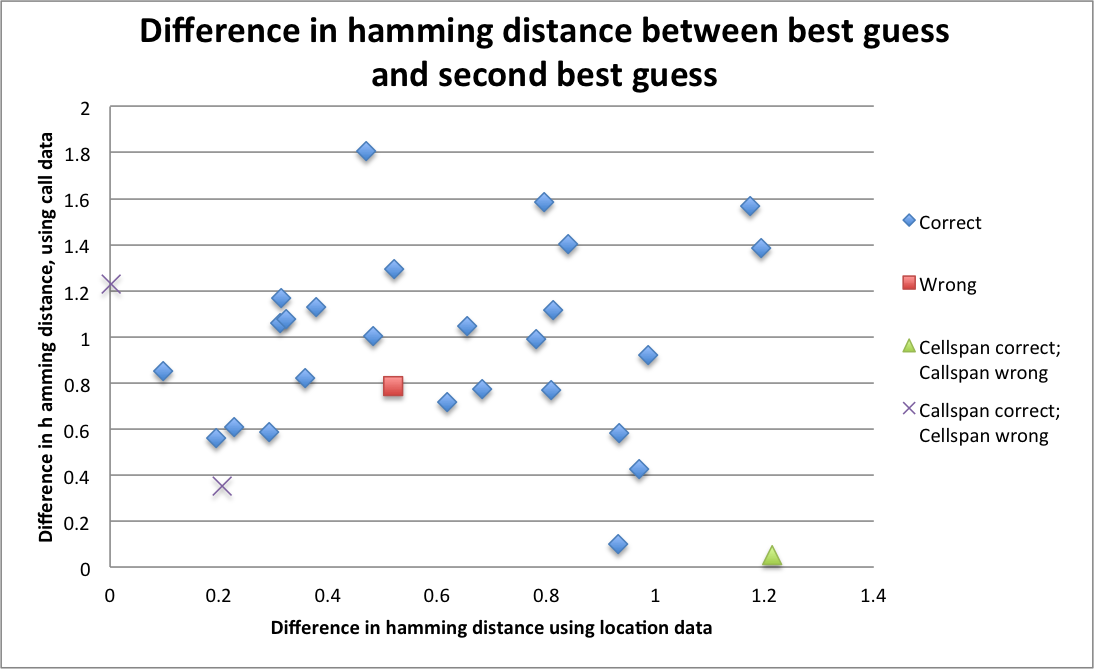
\includegraphics[scale=0.75]{hamming.png}
\end{center}

\section{User similarity: Where does he/she belong?}

The survey data accompanying the users indicates that they are each part of a specific program at MIT. The data distinguishes between:

\begin{itemize}
\item First year graduate students in the Media Lab
\item Upper years graduate students in the Media Lab
\item Undergraduate freshmen in the Media Lab
\item Other undergraduates in the Media Lab
\item Sloan MBA students
\item Media Lab staff
\item Media Lab professors
\end{itemize}

Having found little difference between some of the sub-groups, such as freshmen undergraduate students and other undergraduate students, we have reorganized into the following 4 large categories:

\begin{itemize}
\item Media Lab graduate students (35/97)
\item Media Lab undergraduate students (10/97)
\item Sloan MBA students (27/97)
\item Media Lab staff and professors (6/97)
\end{itemize}

The remaining 19 users were either blank, contained a non-categorical answer (e.g. "Graduated" or "Germany"), or a vague response (e.g. "Student"). 

What we hope to achieve is to answer the question: given any of these users, can we guess which program they belong to simply by comparing their similarity with other users? We attack this question using, as before, location data and call data. 

\subsection{Building profiles}

Whereas in the previous section, we compared the target anonymous user against every other user, here we will compare the target user against various "profiles." In other words, we will compare a user belonging to an unknown academic program to the fictitious typical user representing each of the academic program. 

First, we must build these profiles. We start with the probability distributions for each user, as before. We combine every user known to be in a given program, and take the mean of their distributions. This yields an aggregate distribution which can be used as a profile for that group of users.

Then, we compute the hamming distance between an anonymous user and these four profiles. The highest-ranked profile (with the lowest hamming distance) is selected as the group to which this user belongs. 

\subsection{Location data}

As before, we have the option of using individual cell towers as locations, or of clustering multiple towers into a single location. We present the findings for both approaches. 

\begin{table}[h!]
  \centering
  \begin{tabular}{|l|l|l|}
    \hline
    \textbf{Clusters} & \textbf{Success rate}\\
    \hline
    \hline
    No clustering &  45/73\\
    \hline
    Inflation: 1.4 & 11/73\\
    \hline
    Inflation: 2.0 &  20/73\\
    \hline
    Inflation: 6.0 &  27/73\\
    \hline
  \end{tabular}
  \caption{Success rate with and without clustering}
  \label{table:formatting}
\end{table}

With the largest number of possible locations (no clustering), we were able to achieve a 62\% accuracy. Given that the underlying population contains at least 35 Media Lab graduate students out of 97 candidates, always guessing Media Lab graduate student will give us an accuracy rate of at least 36\%.  As a result, only the approach that preserves all locations without clustering is able to do better than slightly-informed guessing. 

Though we assume the attacker will have knowledge of the underlying distribution, we are able here to do better than simple guessing without using this prior knowledge. One possible explanation is that similarity patterns largely differ from each other. To investigate this hypothesis, we construct the four profiles using every single user, and compute the hamming distance between these profiles. 

\begin{table}[h!]
  \centering
  \begin{tabular}{|l|l|l|l|l|}
    \hline
    \textbf{Profiles} & \textbf{ML grad} & \textbf{ML ugrad} & \textbf{Sloan} & \textbf{ML staff}\\
    \hline
    \hline
    \textbf{ML grad} & - & 1.216 & 1.262 & 1.435\\
    \hline
    \textbf{ML ugrad} & 1.216  & - & 1.432 & 1.540\\
    \hline
    \textbf{Sloan} & 1.262 & 1.432 & - & 1.654\\
    \hline
    \textbf{ML staff} &  1.435 & 1.540 & 1.654& -\\
    \hline
  \end{tabular}
  \caption{Hamming distance between different profiles; no clustering}
  \label{table:formatting}
\end{table}
 
The hypothesis turns out to be inaccurate. The average hamming distance between any anonymous user and its closest profile is 1.544, which suggests that the profiles are not so different from each other. Perhaps there is a way to weight hamming distances using our prior knowledge of the distribution that can help us improve our guessing odds.

\subsection{Call data}

Using 69 users' call data, we were able to identify an anonymous user's academic program at a higher rate than using location data.

\begin{table}[h!]
  \centering
  \begin{tabular}{|l|l|l|l|}
    \hline
    \textbf{Type} & \textbf{Success rate}\\
    \hline
    \hline
    Voice Call &  65/69\\
    \hline
  \end{tabular}
  \caption{Program identification using voice calls}
  \label{table:formatting}
\end{table}

The intuitive explanation behind the higher success rate compared to location is that users in different programs may use the same locations, especially if Sloan is close to the Media Lab, and if undergraduates, graduates, and staff share many of the same facilities. However, users who are in different programs most likely have different social circles: MBAs will interact with each other, graduate students with each other, and so forth. 

To test this intuition, we again computed the hamming distance between the profiles.

\begin{table}[h!]
  \centering
  \begin{tabular}{|l|l|l|l|l|}
    \hline
    \textbf{Profiles} & \textbf{ML grad} & \textbf{ML ugrad} & \textbf{Sloan} & \textbf{ML staff}\\
    \hline
    \hline
    \textbf{ML grad} & - & 1.898 & 1.907 & 1.894\\
    \hline
    \textbf{ML ugrad} & 1.898  & - & 1.913& 1.868\\
    \hline
    \textbf{Sloan} & 1.907 & 1.913 & - & 1.888\\
    \hline
    \textbf{ML staff} &  1.894 & 1.868& 1.888 & -\\
    \hline
  \end{tabular}
  \caption{Hamming distance between different profiles}
  \label{table:formatting}
\end{table}

In this case, our hypothesis appears to be true. The hamming distances between their phone call distributions are higher by roughly 0.4-0.6, compared to the hamming distances between the profiles' location distributions. This difference may account for the increased accuracy in the results.

\section{Choosing friends: Time is friendship}

Finally, we want to investigate whether it is possible to determine friendship between users by using location data. Namely, we hope to discover whether there is a relationship between the amount of time spent in the same location, and the likelihood of friendship between the two users. 

\subsection{Deliberate plans}

Originally, we had hoped to count the amount of time spent in a deliberately planned meeting, i.e. the two users agreed to spend time together at a location, in contrast to two people simply sitting in a lecture together. The approach would be to determine whether short phone calls were made before or at the start of a session where two users were located at the same celltower. Unfortunately, there was no data to support this strategy, as the data set provided no way of reconciling phonenumber\_oids and person\_oids; therefore we had no straightforward way of discovering whether two users spoke to each other over the phone.

\subsection{Chance encounters?}
As a result, we simply have a record of how much time each pair of users spent together at any given cell tower. From the perspective of user i, each other user j is ranked in terms of how much time user j and user i have spent at the same cell tower. We hypothesize that the higher-ranked user j is, the more likely it is that i has reported j to be a friend. 
\subsection{Algorithm}
Below are steps used to tally the amount of time users i and j have spent together. 
\begin{itemize}
\item Take the two sets of location data, sorted by ascending time.
\item Start at the first entry of both logs (counters set to 0).
\item If the two entries do not overlap, increment the counter referring to the earlier record, until it catches up.
\item If the two entries overlap, check whether the location is the same, and record the duration of the overlap if the location is the same. Then increment the counter for the earlier of the 2 entries.
\item Repeat these steps and walk along both logs until one is exhausted.
\end{itemize}

This method is linear in the number of entries for each pair. 

\subsection{Metric}

There are 62 recorded pairs of friends in the data set that are usable. Usable means that the conversion from the SQL person\_oids to the MATLAB network IDs was successful, and that there is location data during the school year available. 

To test whether we are able to identify friends based on amount of time spent together, we randomly selected another 62 pairs at random and made sure that these 62 did not duplicate existing pairs and did not already belong to the reported set of friends. 

For each pair (i, j), we computed the rank of j from the perspective of user i. The more time i and j spend together, the higher the ranking. We then gathered the 62 pairs with the highest rankings, and guessed that these are the friend pairs.

\subsection{Results}

We succesfully identified 33 of the 62 pairs of friends. An entirely random guess is expected to identify half of the friends, 31, and so our algorithm does no better than a random guess. 

Therefore, it seems that the amount of time spent together is too simplistic of a metric. There are many non-friend pairs who must spend time together due to practical reasons imposed by the education system and our method was unable to separate friends from acquaintances.

One further avenue for exploration would be to rank not based on amount of time spent together, but the number of shared locations. The intuition behind this approach is that an individual sees his or her colleagues and classmates in a number of fixed locations, but will be with friends in a variety of locations. 

\section{Conclusion}

A great deal of information can be inferred from the data on cell phone usage and on user location. Each individual's pattern is unique enough that we can generally identify the user in question, and similarities between groups of users can, in the aggregate, characterize the group as a whole. Friendships prove to be more elusive, as there is a significant amount of noise: friendship is only one of many reasons that explain proximity, and it is difficult to distinguish between the different causes by using a simple metric such as amount of time spent together. Nevertheless, the conclusions drawn in this paper should provide further evidence that it has become increasingly difficult to protect user privacy in the information age. 

\end{document}

